\chapter{Definitionen}
\label{ch:chapter02}
Dieses Kapitel erklärt und beschreibt einige der zentralen Begriffe zum Thema des Hostes und der Berechtigungstrukturen.
Dadurch soll der Leser ein Grundverständnis erhalten, um die folgenden Kapitel zu verstehen.

%
% Section: Der erste Abschnitt
%
\section{Begriffserklärung}
\label{sec:Bergriff}

\subsection{Host/Mainframe}
\label{sec:Host}
Der Host oder als auch Mainframe bekannt ist ein Komplex aus verschiedenen Hochleistungscomputern.
Der Anbieter "`IBM"' definiert diesen dabei wie folgt: 
\newline
\newline
\textit{"`At their core, mainframes are high-performance computers with large amounts of memory and processors that process billions of simple calculations and transactions in real time."'} \cite{Mainframe}
\newline
\newline
Oder übersetzt:
\newline
\newline
\textit{"`Im Kern besteht der Mainframe aus Hochleistungsrechnern, welche über einen großen Speicher verfügen, und in der Lage sind Milliarden von einfachen Prozessen und Transaktion in Echtzeit durch zu führen."'} \cite{Mainframe}
\newline
\newline
Dabei spielt der Mainframe eine wichtige Rolle in der finanz Industrie, welche über widerstandsfähige, sichere und agilitäte Server benötigen.
Dies ist der Fall, weil die finanz Industrie über viele sensible Daten verfügt.
Daher müssen die Server sicher und widerstandfähig sein, damit diese Daten nicht verloren gehen oder geklaut werden.
Zudem müssen die Server agil sein, da die Technology und die Regulierungen um den Mainframe sich steht ändern und daher dieser auf dem neuesten Stand sein muss.
Dieser muss nämlich die Regularien vom \ac{VAIT} erfüllen die von der \ac{BaFin} aufgestellt werden.
Diese soll eine konsistente IT-Strategie vorgeben an welche sich die Unternehmen halten müssen. \cite{Vait}

\subsection{Berechtigung}
\label{sec:Berechtigung}
Dabei definiert die \ac{NIST}, welche eine Institution von amerikanische Regierung ist, Berechtigungen wie folgt:
\newline
\newline
\textit{"`The right or a permission that is granted to a system entity to access a system resource."'} \cite{Auth}
\newline
\newline
Dies bedeutet:
\newline
\newline
\textit{"`Das Recht oder die Erlaubnis haben, um auf System Ressourcen einer Systemeinheit zu zugreifen."'} \cite{Mainframe}
\newline
\newline
Im Kontext des Mainframebereiches betrifft dies hauptsächlich das Betrachten und Zugreifen von Dialogmasken bei der Helvetia.
\begin{figure}[h!]
 \centering
 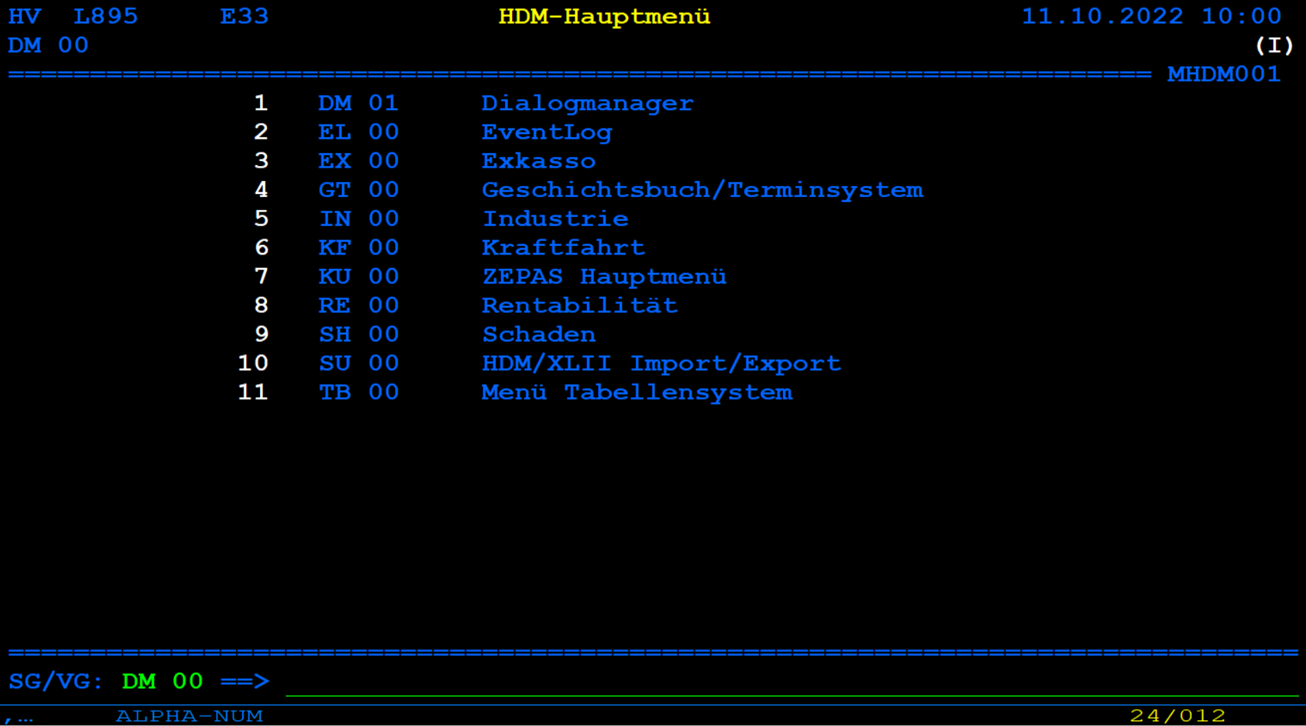
\includegraphics[width=1\textwidth]{gfx/Picture/Dialog.PNG}
 \caption{Beispiel Dialogmaske}
 \label{fig:Dial}
\end{figure}
Die Graphik (\ref{fig:Dial}) zeigt ein solches Dialogmaske.
An hand dieser Dialogmaske kann man erkennen, dass der Nutzer L895 für die aufgezählten weiteren Dialogmasken (EL 00, EX 00,...) zumindest die Leseberechtigung hat.
Zudem hat dieser die Schreibberechtigungen auf die Dialogmaske DM 00, da dieser sich in dieser Maske aufhält. 
\newline
\newline
\begin{figure}[h!]
 \centering
 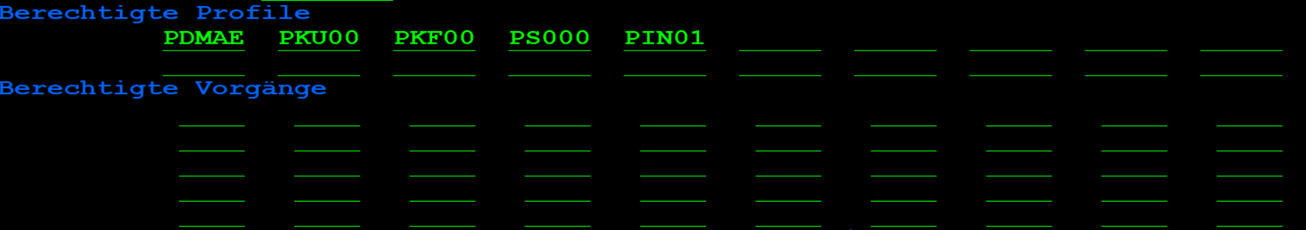
\includegraphics[width=1\textwidth]{gfx/Picture/Berechtigung.PNG}
 \caption{Berechtigungsdialogmaske}
 \label{fig:Berch}
\end{figure}
In dieser Graphik (\ref{fig:Berch}) kann man die Profile und individuellen Berechtigungen sehen, die der Nutzer L895 besitzt.
Dabei sind Profile Container für Berechtigungen.
\subsection{Berechtigungsstruktur}
\label{sec:Berechtigungsstruktur}
Phasellus ut ipsum nulla, vitae venenatis augue. Suspendisse potenti. Mauris suscipit justo a dolor laoreet lacinia. Pellentesque habitant morbi tristique senectus et netus et malesuada fames ac turpis egestas. Aliquam commodo commodo dui, nec auctor mi malesuada et. Aenean tortor erat, semper eu ullamcorper non, dignissim sed lectus. Praesent et pretium leo.

\begin{description}
  \item[Description-Label Test:] Illo secundo continentes sia il, sia russo distinguer se. Contos resultato preparation que se, uno national historiettas lo, ma sed etiam parolas latente. Ma unic quales sia. Pan in patre altere summario, le pro latino resultato.
  \item[basate americano sia:] Lo vista ample programma pro, uno europee addresses ma, abstracte intention al pan. Nos duce infra publicava le. Es que historia encyclopedia, sed terra celos avantiate in. Su pro effortio appellate, o.
  \item[Cras venenatis:] Purus et posuere lacinia, nisl sapien dapibus metus, a ornare enim odio in ipsum. Quisque imperdiet nibh metus, in fringilla tellus. Duis varius dui eget orci commodo ac sollicitudin est placerat. Cras varius tincidunt arcu, quis imperdiet nibh rhoncus vel. Sed non justo orci, non accumsan felis. Maecenas condimentum convallis. 
\end{description}
Tu uno veni americano sanctificate. Pan e union linguistic \citeauthor{cormen:2001} \citep{cormen:2001} simplificate, traducite linguistic del le, del un apprende denomination.

\section{Vorstellung der Methoden}
\label{sec:Bergriff}

\subsection{IAM}
\label{subsec:background:first_section:first_subsection}
Uno pote summario methodicamente al, uso debe nomina hereditage ma. Iala rapide ha del, ma nos esser parlar. Maximo dictionario sed al. Aenean posuere, enim in ultricies facilisis, ligula lacus eleifend eros, accumsan commodo metus justo placerat justo. Donec sit amet mauris dolor, at imperdiet lacus. In laoreet pretium condimentum. Proin ut varius diam. Fusce ipsum ipsum, elementum id porttitor at, pharetra congue nisi.

\subsection{ICAM}
\label{subsec:background:first_section:first_subsection}
Uno pote summario methodicamente al, uso debe nomina hereditage ma. Iala rapide ha del, ma nos esser parlar. Maximo dictionario sed al. Aenean posuere, enim in ultricies facilisis, ligula lacus eleifend eros, accumsan commodo metus justo placerat justo. Donec sit amet mauris dolor, at imperdiet lacus. In laoreet pretium condimentum. Proin ut varius diam. Fusce ipsum ipsum, elementum id porttitor at, pharetra congue nisi.
